\section{实验设计与结果}

% 训练过程分析
\begin{frame}{训练过程分析}
    \begin{columns}
        \column{0.5\textwidth}
        \begin{figure}
            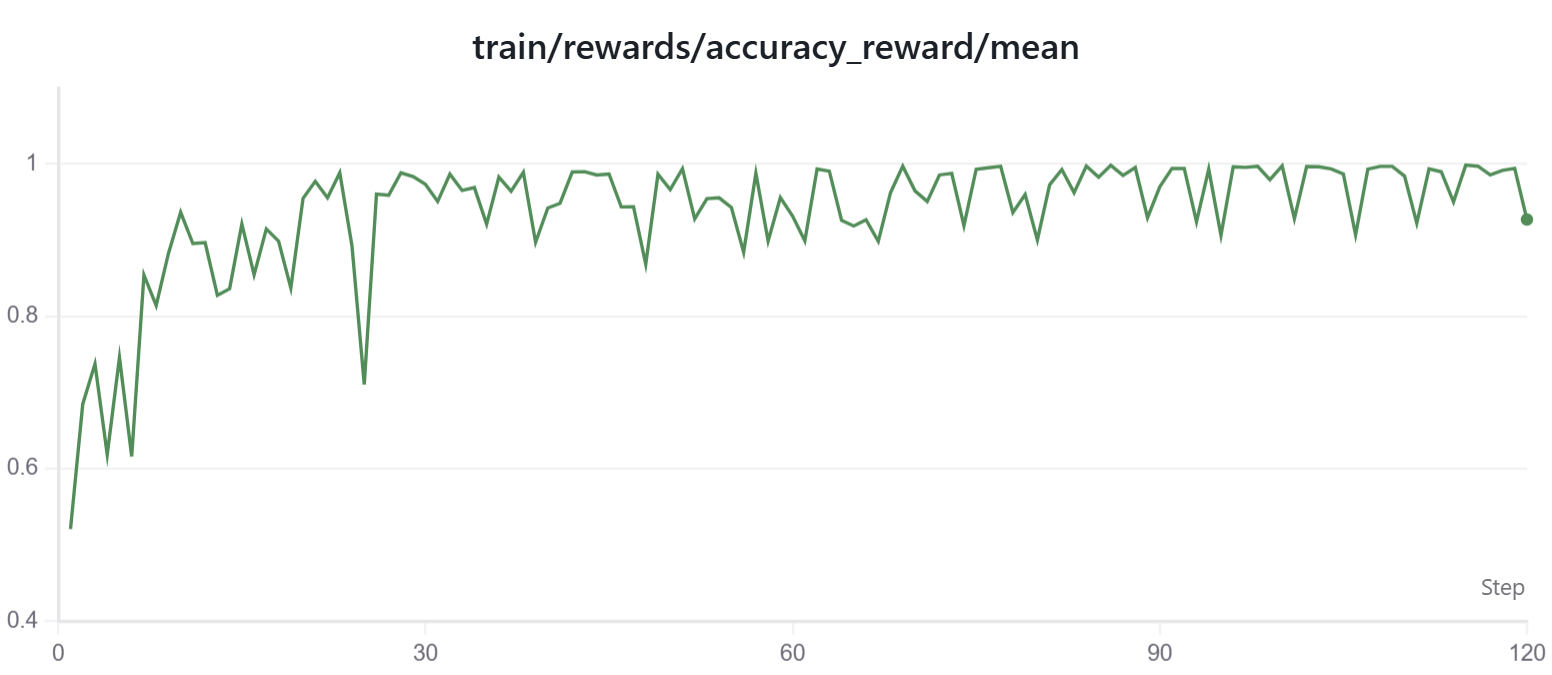
\includegraphics[width=\textwidth]{Images/accuracy_reward.png}
            \caption{准确性奖励变化}
        \end{figure}
        \column{0.5\textwidth}
        \begin{figure}
            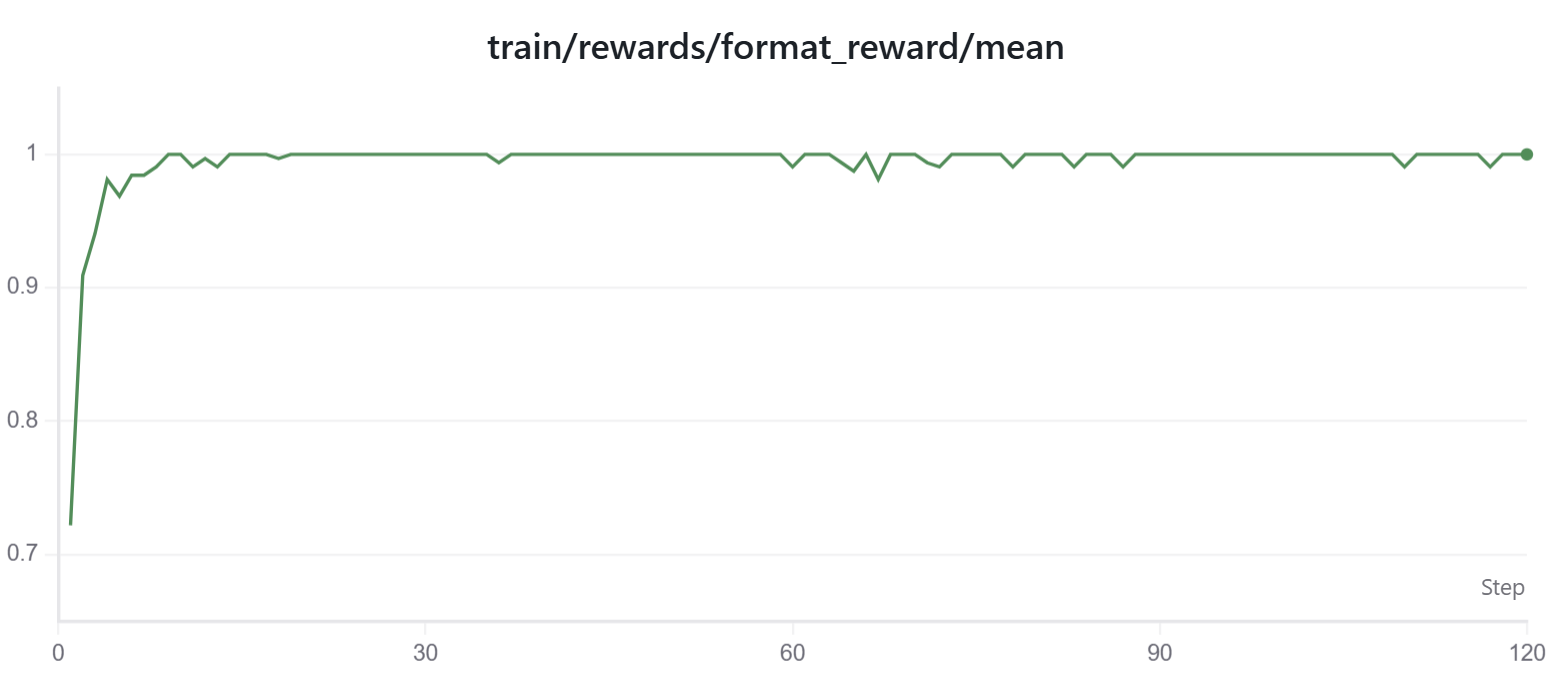
\includegraphics[width=\textwidth]{Images/format_reward.png}
            \caption{格式奖励变化}
        \end{figure}
    \end{columns}
    \begin{itemize}
        \item 准确性奖励:经过60轮训练后趋于稳定
        \item 格式奖励:快速收敛,保持高水平
    \end{itemize}
\end{frame}

% 模型对比分析
\begin{frame}{模型对比分析}
    \begin{columns}
        \column{0.5\textwidth}
        \begin{figure}
            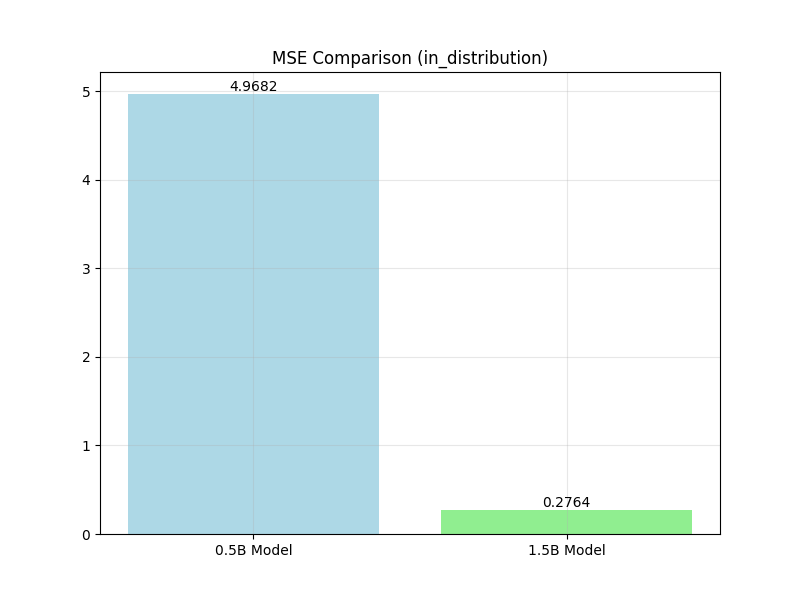
\includegraphics[width=\textwidth]{Images/mse_comparison_in_distribution.png}
            \caption{分布内MSE对比}
        \end{figure}
        \column{0.5\textwidth}
        \begin{figure}
            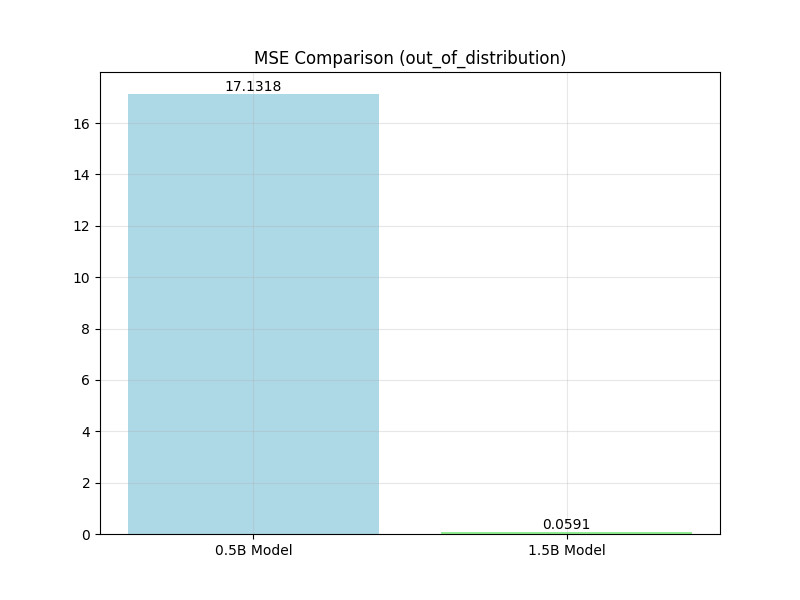
\includegraphics[width=\textwidth]{Images/mse_comparison_out_of_distribution.png}
            \caption{分布外MSE对比}
        \end{figure}
    \end{columns}
    \begin{itemize}
        \item 1.5B模型在两个测试集上都显著优于0.5B模型
        \item 分布外测试集上的优势更为明显
    \end{itemize}
\end{frame}

% 位置误差分析
\begin{frame}{位置误差分析}
    \begin{columns}
        \column{0.5\textwidth}
        \begin{figure}
            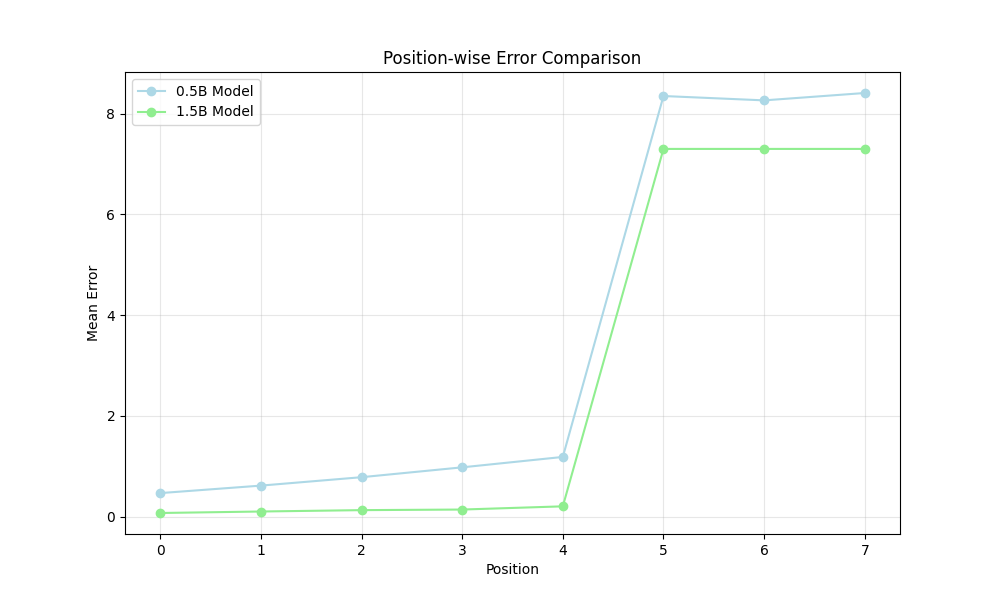
\includegraphics[width=\textwidth]{Images/position_errors_in_distribution.png}
            \caption{分布内位置误差}
        \end{figure}
        \column{0.5\textwidth}
        \begin{figure}
            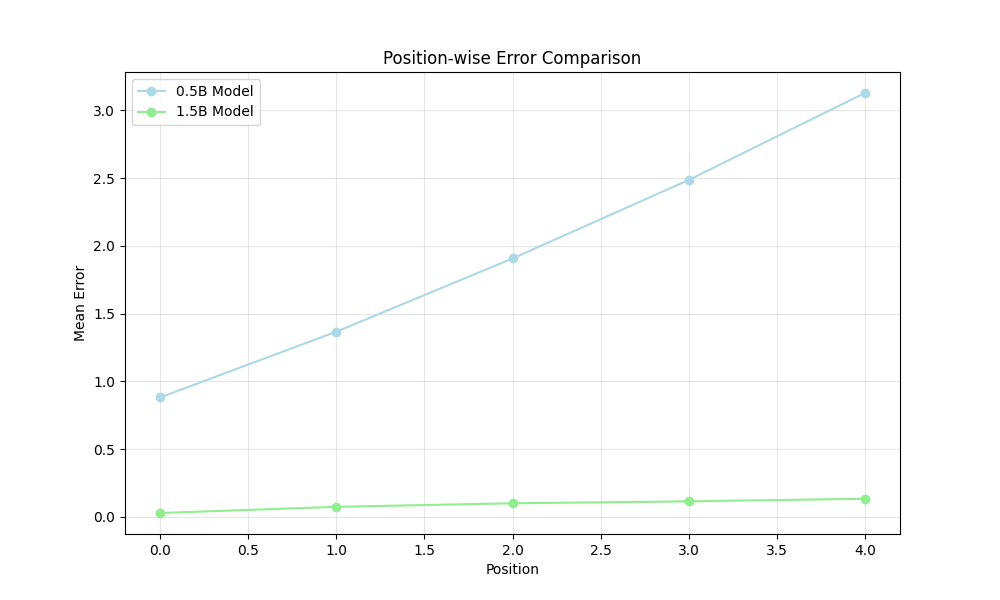
\includegraphics[width=\textwidth]{Images/position_errors_out_of_distribution.png}
            \caption{分布外位置误差}
        \end{figure}
    \end{columns}
    \begin{itemize}
        \item 1.5B模型误差增长更加平缓
        \item 表现出更强的预测稳定性
    \end{itemize}
\end{frame}

% 总结与展望
\begin{frame}{总结与展望}
    \begin{itemize}
        \item \textbf{主要创新点}
        \begin{itemize}
            \item 多维度奖励函数设计
            \item 详细的位置误差分析
            \item 分布内外泛化能力评估
        \end{itemize}
        \vspace{0.3cm}
        \item \textbf{未来工作}
        \begin{itemize}
            \item 扩展到更复杂的运动模式
            \item 优化奖励计算效率
            \item 提升模型泛化能力
        \end{itemize}
    \end{itemize}
\end{frame}

% 结束页
\begin{frame}
    \begin{center}
        \Huge 感谢聆听!
        \vspace{1cm}
        
        \Large Q \& A
    \end{center}
\end{frame}

% \begin{frame}{Referências}
%     \nocite{*}
%     \printbibliography[heading=none]
% \end{frame}